\documentclass[twoside]{book}

% Packages required by doxygen
\usepackage{fixltx2e}
\usepackage{calc}
\usepackage{doxygen}
\usepackage[export]{adjustbox} % also loads graphicx
\usepackage{graphicx}
\usepackage[utf8]{inputenc}
\usepackage{makeidx}
\usepackage{multicol}
\usepackage{multirow}
\PassOptionsToPackage{warn}{textcomp}
\usepackage{textcomp}
\usepackage[nointegrals]{wasysym}
\usepackage[table]{xcolor}

% Font selection
\usepackage[T1]{fontenc}
\usepackage[scaled=.90]{helvet}
\usepackage{courier}
\usepackage{amssymb}
\usepackage{sectsty}
\renewcommand{\familydefault}{\sfdefault}
\allsectionsfont{%
  \fontseries{bc}\selectfont%
  \color{darkgray}%
}
\renewcommand{\DoxyLabelFont}{%
  \fontseries{bc}\selectfont%
  \color{darkgray}%
}
\newcommand{\+}{\discretionary{\mbox{\scriptsize$\hookleftarrow$}}{}{}}

% Page & text layout
\usepackage{geometry}
\geometry{%
  a4paper,%
  top=2.5cm,%
  bottom=2.5cm,%
  left=2.5cm,%
  right=2.5cm%
}
\tolerance=750
\hfuzz=15pt
\hbadness=750
\setlength{\emergencystretch}{15pt}
\setlength{\parindent}{0cm}
\setlength{\parskip}{3ex plus 2ex minus 2ex}
\makeatletter
\renewcommand{\paragraph}{%
  \@startsection{paragraph}{4}{0ex}{-1.0ex}{1.0ex}{%
    \normalfont\normalsize\bfseries\SS@parafont%
  }%
}
\renewcommand{\subparagraph}{%
  \@startsection{subparagraph}{5}{0ex}{-1.0ex}{1.0ex}{%
    \normalfont\normalsize\bfseries\SS@subparafont%
  }%
}
\makeatother

% Headers & footers
\usepackage{fancyhdr}
\pagestyle{fancyplain}
\fancyhead[LE]{\fancyplain{}{\bfseries\thepage}}
\fancyhead[CE]{\fancyplain{}{}}
\fancyhead[RE]{\fancyplain{}{\bfseries\leftmark}}
\fancyhead[LO]{\fancyplain{}{\bfseries\rightmark}}
\fancyhead[CO]{\fancyplain{}{}}
\fancyhead[RO]{\fancyplain{}{\bfseries\thepage}}
\fancyfoot[LE]{\fancyplain{}{}}
\fancyfoot[CE]{\fancyplain{}{}}
\fancyfoot[RE]{\fancyplain{}{\bfseries\scriptsize Generated by Doxygen }}
\fancyfoot[LO]{\fancyplain{}{\bfseries\scriptsize Generated by Doxygen }}
\fancyfoot[CO]{\fancyplain{}{}}
\fancyfoot[RO]{\fancyplain{}{}}
\renewcommand{\footrulewidth}{0.4pt}
\renewcommand{\chaptermark}[1]{%
  \markboth{#1}{}%
}
\renewcommand{\sectionmark}[1]{%
  \markright{\thesection\ #1}%
}

% Indices & bibliography
\usepackage{natbib}
\usepackage[titles]{tocloft}
\setcounter{tocdepth}{3}
\setcounter{secnumdepth}{5}
\makeindex

% Hyperlinks (required, but should be loaded last)
\usepackage{ifpdf}
\ifpdf
  \usepackage[pdftex,pagebackref=true]{hyperref}
\else
  \usepackage[ps2pdf,pagebackref=true]{hyperref}
\fi
\hypersetup{%
  colorlinks=true,%
  linkcolor=blue,%
  citecolor=blue,%
  unicode%
}

% Custom commands
\newcommand{\clearemptydoublepage}{%
  \newpage{\pagestyle{empty}\cleardoublepage}%
}

\usepackage{caption}
\captionsetup{labelsep=space,justification=centering,font={bf},singlelinecheck=off,skip=4pt,position=top}

%===== C O N T E N T S =====

\begin{document}

% Titlepage & ToC
\hypersetup{pageanchor=false,
             bookmarksnumbered=true,
             pdfencoding=unicode
            }
\pagenumbering{alph}
\begin{titlepage}
\vspace*{7cm}
\begin{center}%
{\Large Projeto\+P1 \\[1ex]\large 1.\+0 }\\
\vspace*{1cm}
{\large Generated by Doxygen 1.8.14}\\
\end{center}
\end{titlepage}
\clearemptydoublepage
\pagenumbering{roman}
\tableofcontents
\clearemptydoublepage
\pagenumbering{arabic}
\hypersetup{pageanchor=true}

%--- Begin generated contents ---
\chapter{Hierarchical Index}
\section{Class Hierarchy}
This inheritance list is sorted roughly, but not completely, alphabetically\+:\begin{DoxyCompactList}
\item \contentsline{section}{Mundo}{\pageref{class_mundo}}{}
\item \contentsline{section}{Veiculo}{\pageref{class_veiculo}}{}
\begin{DoxyCompactList}
\item \contentsline{section}{Caminhao}{\pageref{class_caminhao}}{}
\item \contentsline{section}{Carro}{\pageref{class_carro}}{}
\item \contentsline{section}{Moto}{\pageref{class_moto}}{}
\end{DoxyCompactList}
\end{DoxyCompactList}

\chapter{Class Index}
\section{Class List}
Here are the classes, structs, unions and interfaces with brief descriptions\+:\begin{DoxyCompactList}
\item\contentsline{section}{\mbox{\hyperlink{class_caminhao}{Caminhao}} }{\pageref{class_caminhao}}{}
\item\contentsline{section}{\mbox{\hyperlink{class_carro}{Carro}} }{\pageref{class_carro}}{}
\item\contentsline{section}{\mbox{\hyperlink{class_moto}{Moto}} }{\pageref{class_moto}}{}
\item\contentsline{section}{\mbox{\hyperlink{class_mundo}{Mundo}} }{\pageref{class_mundo}}{}
\item\contentsline{section}{\mbox{\hyperlink{class_veiculo}{Veiculo}} }{\pageref{class_veiculo}}{}
\end{DoxyCompactList}

\chapter{File Index}
\section{File List}
Here is a list of all files with brief descriptions\+:\begin{DoxyCompactList}
\item\contentsline{section}{Aplicação/\mbox{\hyperlink{_caminhao_8java}{Caminhao.\+java}} }{\pageref{_caminhao_8java}}{}
\item\contentsline{section}{Aplicação/\mbox{\hyperlink{_carro_8java}{Carro.\+java}} }{\pageref{_carro_8java}}{}
\item\contentsline{section}{Aplicação/\mbox{\hyperlink{_main_8java}{Main.\+java}} }{\pageref{_main_8java}}{}
\item\contentsline{section}{Aplicação/\mbox{\hyperlink{_moto_8java}{Moto.\+java}} }{\pageref{_moto_8java}}{}
\item\contentsline{section}{Aplicação/\mbox{\hyperlink{_mundo_8java}{Mundo.\+java}} }{\pageref{_mundo_8java}}{}
\item\contentsline{section}{Aplicação/\mbox{\hyperlink{_veiculo_8java}{Veiculo.\+java}} }{\pageref{_veiculo_8java}}{}
\end{DoxyCompactList}

\chapter{Class Documentation}
\hypertarget{class_caminhao}{}\section{Caminhao Class Reference}
\label{class_caminhao}\index{Caminhao@{Caminhao}}


Inheritance diagram for Caminhao\+:
\nopagebreak
\begin{figure}[H]
\begin{center}
\leavevmode
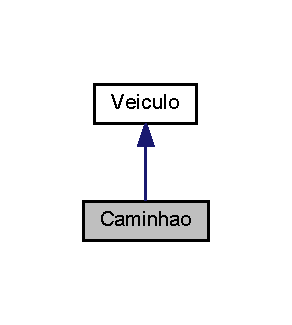
\includegraphics[width=140pt]{class_caminhao__inherit__graph}
\end{center}
\end{figure}


Collaboration diagram for Caminhao\+:
\nopagebreak
\begin{figure}[H]
\begin{center}
\leavevmode
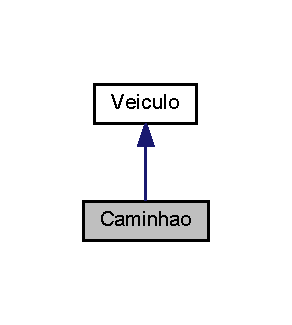
\includegraphics[width=140pt]{class_caminhao__coll__graph}
\end{center}
\end{figure}
\subsection*{Public Member Functions}
\begin{DoxyCompactItemize}
\item 
\mbox{\hyperlink{class_caminhao_af84806c020691e90179569546094dc5a}{Caminhao}} (int \mbox{\hyperlink{class_veiculo_a069917a284297fe5b385258b2afd9ad6}{x}}, int \mbox{\hyperlink{class_veiculo_af25046404db7c2786c0d9e468bb1fb64}{y}}, int \mbox{\hyperlink{class_veiculo_a2edf5e3132b1c2504c441dc095dc7e0e}{velocidade}})
\end{DoxyCompactItemize}
\subsection*{Additional Inherited Members}


\subsection{Constructor \& Destructor Documentation}
\mbox{\Hypertarget{class_caminhao_af84806c020691e90179569546094dc5a}\label{class_caminhao_af84806c020691e90179569546094dc5a}} 
\index{Caminhao@{Caminhao}!Caminhao@{Caminhao}}
\index{Caminhao@{Caminhao}!Caminhao@{Caminhao}}
\subsubsection{\texorpdfstring{Caminhao()}{Caminhao()}}
{\footnotesize\ttfamily Caminhao.\+Caminhao (\begin{DoxyParamCaption}\item[{int}]{x,  }\item[{int}]{y,  }\item[{int}]{velocidade }\end{DoxyParamCaption})}



The documentation for this class was generated from the following file\+:\begin{DoxyCompactItemize}
\item 
Aplicação/\mbox{\hyperlink{_caminhao_8java}{Caminhao.\+java}}\end{DoxyCompactItemize}

\hypertarget{class_carro}{}\section{Carro Class Reference}
\label{class_carro}\index{Carro@{Carro}}


Inheritance diagram for Carro\+:
\nopagebreak
\begin{figure}[H]
\begin{center}
\leavevmode
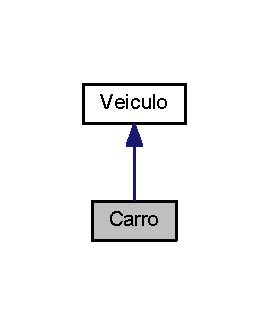
\includegraphics[width=129pt]{class_carro__inherit__graph}
\end{center}
\end{figure}


Collaboration diagram for Carro\+:
\nopagebreak
\begin{figure}[H]
\begin{center}
\leavevmode
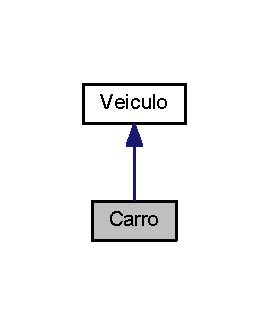
\includegraphics[width=129pt]{class_carro__coll__graph}
\end{center}
\end{figure}
\subsection*{Public Member Functions}
\begin{DoxyCompactItemize}
\item 
\mbox{\hyperlink{class_carro_a5637631ba38ec32090b43e8932071695}{Carro}} (int \mbox{\hyperlink{class_veiculo_a069917a284297fe5b385258b2afd9ad6}{x}}, int \mbox{\hyperlink{class_veiculo_af25046404db7c2786c0d9e468bb1fb64}{y}}, int \mbox{\hyperlink{class_veiculo_a2edf5e3132b1c2504c441dc095dc7e0e}{velocidade}})
\end{DoxyCompactItemize}
\subsection*{Additional Inherited Members}


\subsection{Constructor \& Destructor Documentation}
\mbox{\Hypertarget{class_carro_a5637631ba38ec32090b43e8932071695}\label{class_carro_a5637631ba38ec32090b43e8932071695}} 
\index{Carro@{Carro}!Carro@{Carro}}
\index{Carro@{Carro}!Carro@{Carro}}
\subsubsection{\texorpdfstring{Carro()}{Carro()}}
{\footnotesize\ttfamily Carro.\+Carro (\begin{DoxyParamCaption}\item[{int}]{x,  }\item[{int}]{y,  }\item[{int}]{velocidade }\end{DoxyParamCaption})}



The documentation for this class was generated from the following file\+:\begin{DoxyCompactItemize}
\item 
Aplicação/\mbox{\hyperlink{_carro_8java}{Carro.\+java}}\end{DoxyCompactItemize}

\hypertarget{class_moto}{}\section{Moto Class Reference}
\label{class_moto}\index{Moto@{Moto}}


Inheritance diagram for Moto\+:
\nopagebreak
\begin{figure}[H]
\begin{center}
\leavevmode
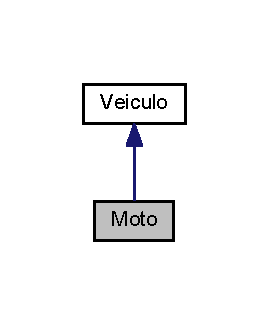
\includegraphics[width=129pt]{class_moto__inherit__graph}
\end{center}
\end{figure}


Collaboration diagram for Moto\+:
\nopagebreak
\begin{figure}[H]
\begin{center}
\leavevmode
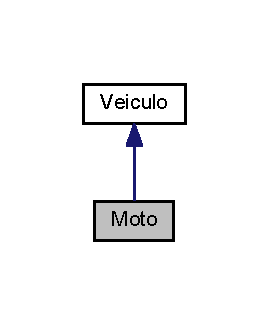
\includegraphics[width=129pt]{class_moto__coll__graph}
\end{center}
\end{figure}
\subsection*{Public Member Functions}
\begin{DoxyCompactItemize}
\item 
\mbox{\hyperlink{class_moto_ab81ca0fb4282aa5bd34f9b9d6902bdbb}{Moto}} (int \mbox{\hyperlink{class_veiculo_a069917a284297fe5b385258b2afd9ad6}{x}}, int \mbox{\hyperlink{class_veiculo_af25046404db7c2786c0d9e468bb1fb64}{y}}, int \mbox{\hyperlink{class_veiculo_a2edf5e3132b1c2504c441dc095dc7e0e}{velocidade}})
\end{DoxyCompactItemize}
\subsection*{Additional Inherited Members}


\subsection{Constructor \& Destructor Documentation}
\mbox{\Hypertarget{class_moto_ab81ca0fb4282aa5bd34f9b9d6902bdbb}\label{class_moto_ab81ca0fb4282aa5bd34f9b9d6902bdbb}} 
\index{Moto@{Moto}!Moto@{Moto}}
\index{Moto@{Moto}!Moto@{Moto}}
\subsubsection{\texorpdfstring{Moto()}{Moto()}}
{\footnotesize\ttfamily Moto.\+Moto (\begin{DoxyParamCaption}\item[{int}]{x,  }\item[{int}]{y,  }\item[{int}]{velocidade }\end{DoxyParamCaption})}



The documentation for this class was generated from the following file\+:\begin{DoxyCompactItemize}
\item 
Aplicação/\mbox{\hyperlink{_moto_8java}{Moto.\+java}}\end{DoxyCompactItemize}

\hypertarget{class_mundo}{}\section{Mundo Class Reference}
\label{class_mundo}\index{Mundo@{Mundo}}
\subsection*{Public Member Functions}
\begin{DoxyCompactItemize}
\item 
void \mbox{\hyperlink{class_mundo_af3c85a96da0920ffc66893bf8cc4d055}{cria\+Mundo}} (Array\+List$<$ \mbox{\hyperlink{class_moto}{Moto}} $>$ b, Array\+List$<$ \mbox{\hyperlink{class_carro}{Carro}} $>$ c, Array\+List$<$ \mbox{\hyperlink{class_caminhao}{Caminhao}} $>$ t)
\item 
void \mbox{\hyperlink{class_mundo_a73f12c49f3b9a107eec95698d4e52549}{checa\+Fabrica}} (Array\+List$<$ \mbox{\hyperlink{class_moto}{Moto}} $>$ b, Array\+List$<$ \mbox{\hyperlink{class_carro}{Carro}} $>$ c, Array\+List$<$ \mbox{\hyperlink{class_caminhao}{Caminhao}} $>$ t)
\begin{DoxyCompactList}\small\item\em detecta fabrica e duplica objeto \end{DoxyCompactList}\item 
void \mbox{\hyperlink{class_mundo_a7a5e6f53aa4ecce473987615c08e3207}{colisao}} (Array\+List$<$ \mbox{\hyperlink{class_moto}{Moto}} $>$ b, Array\+List$<$ \mbox{\hyperlink{class_carro}{Carro}} $>$ c, Array\+List$<$ \mbox{\hyperlink{class_caminhao}{Caminhao}} $>$ t)
\begin{DoxyCompactList}\small\item\em colisoes \end{DoxyCompactList}\item 
void \mbox{\hyperlink{class_mundo_a063aff787cf37c4f6461c825a5f6be26}{imprime\+Mundo}} (Array\+List$<$ \mbox{\hyperlink{class_moto}{Moto}} $>$ b, Array\+List$<$ \mbox{\hyperlink{class_carro}{Carro}} $>$ c, Array\+List$<$ \mbox{\hyperlink{class_caminhao}{Caminhao}} $>$ t)
\end{DoxyCompactItemize}


\subsection{Member Function Documentation}
\mbox{\Hypertarget{class_mundo_a73f12c49f3b9a107eec95698d4e52549}\label{class_mundo_a73f12c49f3b9a107eec95698d4e52549}} 
\index{Mundo@{Mundo}!checa\+Fabrica@{checa\+Fabrica}}
\index{checa\+Fabrica@{checa\+Fabrica}!Mundo@{Mundo}}
\subsubsection{\texorpdfstring{checa\+Fabrica()}{checaFabrica()}}
{\footnotesize\ttfamily void Mundo.\+checa\+Fabrica (\begin{DoxyParamCaption}\item[{Array\+List$<$ \mbox{\hyperlink{class_moto}{Moto}} $>$}]{b,  }\item[{Array\+List$<$ \mbox{\hyperlink{class_carro}{Carro}} $>$}]{c,  }\item[{Array\+List$<$ \mbox{\hyperlink{class_caminhao}{Caminhao}} $>$}]{t }\end{DoxyParamCaption})}



detecta fabrica e duplica objeto 

\mbox{\Hypertarget{class_mundo_a7a5e6f53aa4ecce473987615c08e3207}\label{class_mundo_a7a5e6f53aa4ecce473987615c08e3207}} 
\index{Mundo@{Mundo}!colisao@{colisao}}
\index{colisao@{colisao}!Mundo@{Mundo}}
\subsubsection{\texorpdfstring{colisao()}{colisao()}}
{\footnotesize\ttfamily void Mundo.\+colisao (\begin{DoxyParamCaption}\item[{Array\+List$<$ \mbox{\hyperlink{class_moto}{Moto}} $>$}]{b,  }\item[{Array\+List$<$ \mbox{\hyperlink{class_carro}{Carro}} $>$}]{c,  }\item[{Array\+List$<$ \mbox{\hyperlink{class_caminhao}{Caminhao}} $>$}]{t }\end{DoxyParamCaption})}



colisoes 

\mbox{\Hypertarget{class_mundo_af3c85a96da0920ffc66893bf8cc4d055}\label{class_mundo_af3c85a96da0920ffc66893bf8cc4d055}} 
\index{Mundo@{Mundo}!cria\+Mundo@{cria\+Mundo}}
\index{cria\+Mundo@{cria\+Mundo}!Mundo@{Mundo}}
\subsubsection{\texorpdfstring{cria\+Mundo()}{criaMundo()}}
{\footnotesize\ttfamily void Mundo.\+cria\+Mundo (\begin{DoxyParamCaption}\item[{Array\+List$<$ \mbox{\hyperlink{class_moto}{Moto}} $>$}]{b,  }\item[{Array\+List$<$ \mbox{\hyperlink{class_carro}{Carro}} $>$}]{c,  }\item[{Array\+List$<$ \mbox{\hyperlink{class_caminhao}{Caminhao}} $>$}]{t }\end{DoxyParamCaption})}

$<$ i=linhas

$<$ j=colunas

$<$ todo mundo zero

$<$ primeira linha de 1

$<$ ultima linha de 1

$<$ ultima coluna de 1

$<$ primeira coluna de 1

$<$ joga caminhoes aleatoriamente no mundo

$<$ joga motos aleatoriamente no mundo

$<$ joga carros aleatoriamente no mundo \mbox{\Hypertarget{class_mundo_a063aff787cf37c4f6461c825a5f6be26}\label{class_mundo_a063aff787cf37c4f6461c825a5f6be26}} 
\index{Mundo@{Mundo}!imprime\+Mundo@{imprime\+Mundo}}
\index{imprime\+Mundo@{imprime\+Mundo}!Mundo@{Mundo}}
\subsubsection{\texorpdfstring{imprime\+Mundo()}{imprimeMundo()}}
{\footnotesize\ttfamily void Mundo.\+imprime\+Mundo (\begin{DoxyParamCaption}\item[{Array\+List$<$ \mbox{\hyperlink{class_moto}{Moto}} $>$}]{b,  }\item[{Array\+List$<$ \mbox{\hyperlink{class_carro}{Carro}} $>$}]{c,  }\item[{Array\+List$<$ \mbox{\hyperlink{class_caminhao}{Caminhao}} $>$}]{t }\end{DoxyParamCaption})}



The documentation for this class was generated from the following file\+:\begin{DoxyCompactItemize}
\item 
Aplicação/\mbox{\hyperlink{_mundo_8java}{Mundo.\+java}}\end{DoxyCompactItemize}

\hypertarget{class_veiculo}{}\section{Veiculo Class Reference}
\label{class_veiculo}\index{Veiculo@{Veiculo}}


Inheritance diagram for Veiculo\+:
\nopagebreak
\begin{figure}[H]
\begin{center}
\leavevmode
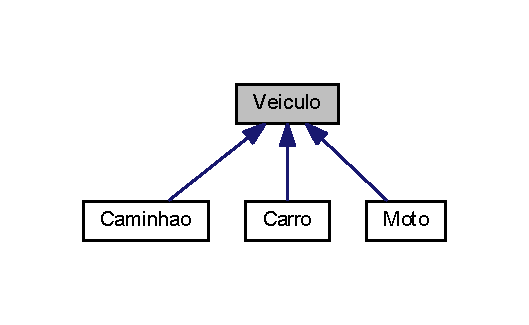
\includegraphics[width=254pt]{class_veiculo__inherit__graph}
\end{center}
\end{figure}
\subsection*{Public Member Functions}
\begin{DoxyCompactItemize}
\item 
\mbox{\hyperlink{class_veiculo_aa4854ce911d37f725ce5374c1dee62af}{Veiculo}} (int \mbox{\hyperlink{class_veiculo_a069917a284297fe5b385258b2afd9ad6}{x}}, int \mbox{\hyperlink{class_veiculo_af25046404db7c2786c0d9e468bb1fb64}{y}}, int \mbox{\hyperlink{class_veiculo_a2edf5e3132b1c2504c441dc095dc7e0e}{velocidade}})
\begin{DoxyCompactList}\small\item\em construtor parametrizado \end{DoxyCompactList}\item 
void \mbox{\hyperlink{class_veiculo_a7c9b89bb072fedf9c24d1586ec31101b}{set\+Velo}} (int \mbox{\hyperlink{class_veiculo_a2edf5e3132b1c2504c441dc095dc7e0e}{velocidade}})
\begin{DoxyCompactList}\small\item\em set da velocidade \end{DoxyCompactList}\item 
void \mbox{\hyperlink{class_veiculo_a84b2207a013e6cd869959b73a93864b8}{setX}} (int \mbox{\hyperlink{class_veiculo_a069917a284297fe5b385258b2afd9ad6}{x}})
\begin{DoxyCompactList}\small\item\em set do x \end{DoxyCompactList}\item 
void \mbox{\hyperlink{class_veiculo_a57cb54424b47643d8b388c72dbaf43b1}{setY}} (int \mbox{\hyperlink{class_veiculo_af25046404db7c2786c0d9e468bb1fb64}{y}})
\begin{DoxyCompactList}\small\item\em set do y \end{DoxyCompactList}\item 
void \mbox{\hyperlink{class_veiculo_ae9a07a54a5824a9e8cace2c742034956}{set\+Fabrica}} (boolean \mbox{\hyperlink{class_veiculo_a23d377a69bdf558ebedb5bc35dcdebf5}{fabrica}})
\begin{DoxyCompactList}\small\item\em set da fabrica \end{DoxyCompactList}\item 
int \mbox{\hyperlink{class_veiculo_aed4b192929f7efd2234059f139bb29df}{get\+Velo}} ()
\begin{DoxyCompactList}\small\item\em get da velocidade \end{DoxyCompactList}\item 
int \mbox{\hyperlink{class_veiculo_a235b29e1e25ec8c769b20fb2aeba8404}{getX}} ()
\begin{DoxyCompactList}\small\item\em get do x \end{DoxyCompactList}\item 
int \mbox{\hyperlink{class_veiculo_a06b2a923e51186673a016f75d10363d3}{getY}} ()
\begin{DoxyCompactList}\small\item\em get do y \end{DoxyCompactList}\item 
boolean \mbox{\hyperlink{class_veiculo_a6447f0eeb99399f1f96e835c22a88479}{get\+Fabrica}} ()
\begin{DoxyCompactList}\small\item\em get da fabrica \end{DoxyCompactList}\item 
void \mbox{\hyperlink{class_veiculo_a3341b0ed6b4d34db990a31f7a499ae80}{move}} ()
\item 
void \mbox{\hyperlink{class_veiculo_aa0233fb9ba21481a8f43780270a5f9ec}{checa\+Fabrica}} ()
\end{DoxyCompactItemize}
\subsection*{Protected Attributes}
\begin{DoxyCompactItemize}
\item 
int \mbox{\hyperlink{class_veiculo_a069917a284297fe5b385258b2afd9ad6}{x}}
\begin{DoxyCompactList}\small\item\em linha \end{DoxyCompactList}\item 
int \mbox{\hyperlink{class_veiculo_af25046404db7c2786c0d9e468bb1fb64}{y}}
\begin{DoxyCompactList}\small\item\em coluna \end{DoxyCompactList}\item 
int \mbox{\hyperlink{class_veiculo_a2edf5e3132b1c2504c441dc095dc7e0e}{velocidade}}
\begin{DoxyCompactList}\small\item\em velocidade \end{DoxyCompactList}\item 
boolean \mbox{\hyperlink{class_veiculo_a23d377a69bdf558ebedb5bc35dcdebf5}{fabrica}}
\begin{DoxyCompactList}\small\item\em pra detectar se passa ou nao pela fabrica \end{DoxyCompactList}\end{DoxyCompactItemize}


\subsection{Constructor \& Destructor Documentation}
\mbox{\Hypertarget{class_veiculo_aa4854ce911d37f725ce5374c1dee62af}\label{class_veiculo_aa4854ce911d37f725ce5374c1dee62af}} 
\index{Veiculo@{Veiculo}!Veiculo@{Veiculo}}
\index{Veiculo@{Veiculo}!Veiculo@{Veiculo}}
\subsubsection{\texorpdfstring{Veiculo()}{Veiculo()}}
{\footnotesize\ttfamily Veiculo.\+Veiculo (\begin{DoxyParamCaption}\item[{int}]{x,  }\item[{int}]{y,  }\item[{int}]{velocidade }\end{DoxyParamCaption})}



construtor parametrizado 



\subsection{Member Function Documentation}
\mbox{\Hypertarget{class_veiculo_aa0233fb9ba21481a8f43780270a5f9ec}\label{class_veiculo_aa0233fb9ba21481a8f43780270a5f9ec}} 
\index{Veiculo@{Veiculo}!checa\+Fabrica@{checa\+Fabrica}}
\index{checa\+Fabrica@{checa\+Fabrica}!Veiculo@{Veiculo}}
\subsubsection{\texorpdfstring{checa\+Fabrica()}{checaFabrica()}}
{\footnotesize\ttfamily void Veiculo.\+checa\+Fabrica (\begin{DoxyParamCaption}{ }\end{DoxyParamCaption})}

checa se na posição é área da fábrica, se sim faz atributo fabrica ser true\mbox{\Hypertarget{class_veiculo_a6447f0eeb99399f1f96e835c22a88479}\label{class_veiculo_a6447f0eeb99399f1f96e835c22a88479}} 
\index{Veiculo@{Veiculo}!get\+Fabrica@{get\+Fabrica}}
\index{get\+Fabrica@{get\+Fabrica}!Veiculo@{Veiculo}}
\subsubsection{\texorpdfstring{get\+Fabrica()}{getFabrica()}}
{\footnotesize\ttfamily boolean Veiculo.\+get\+Fabrica (\begin{DoxyParamCaption}{ }\end{DoxyParamCaption})}



get da fabrica 

\mbox{\Hypertarget{class_veiculo_aed4b192929f7efd2234059f139bb29df}\label{class_veiculo_aed4b192929f7efd2234059f139bb29df}} 
\index{Veiculo@{Veiculo}!get\+Velo@{get\+Velo}}
\index{get\+Velo@{get\+Velo}!Veiculo@{Veiculo}}
\subsubsection{\texorpdfstring{get\+Velo()}{getVelo()}}
{\footnotesize\ttfamily int Veiculo.\+get\+Velo (\begin{DoxyParamCaption}{ }\end{DoxyParamCaption})}



get da velocidade 

\mbox{\Hypertarget{class_veiculo_a235b29e1e25ec8c769b20fb2aeba8404}\label{class_veiculo_a235b29e1e25ec8c769b20fb2aeba8404}} 
\index{Veiculo@{Veiculo}!getX@{getX}}
\index{getX@{getX}!Veiculo@{Veiculo}}
\subsubsection{\texorpdfstring{get\+X()}{getX()}}
{\footnotesize\ttfamily int Veiculo.\+getX (\begin{DoxyParamCaption}{ }\end{DoxyParamCaption})}



get do x 

\mbox{\Hypertarget{class_veiculo_a06b2a923e51186673a016f75d10363d3}\label{class_veiculo_a06b2a923e51186673a016f75d10363d3}} 
\index{Veiculo@{Veiculo}!getY@{getY}}
\index{getY@{getY}!Veiculo@{Veiculo}}
\subsubsection{\texorpdfstring{get\+Y()}{getY()}}
{\footnotesize\ttfamily int Veiculo.\+getY (\begin{DoxyParamCaption}{ }\end{DoxyParamCaption})}



get do y 

\mbox{\Hypertarget{class_veiculo_a3341b0ed6b4d34db990a31f7a499ae80}\label{class_veiculo_a3341b0ed6b4d34db990a31f7a499ae80}} 
\index{Veiculo@{Veiculo}!move@{move}}
\index{move@{move}!Veiculo@{Veiculo}}
\subsubsection{\texorpdfstring{move()}{move()}}
{\footnotesize\ttfamily void Veiculo.\+move (\begin{DoxyParamCaption}{ }\end{DoxyParamCaption})}

$<$ gera numero aletorio entre 0-\/3

$<$ vai pra cima

$<$ se y bater na borda de cima, volta pra baixo

$<$ vai pra direita

$<$ se x chegar na borda direita, volta pra esquerda

$<$ move pra baixo

$<$ se y chegar na borda de baixo, volta pro alto

$<$ vai pra esquerda

$<$ se x chegar na borda esquerda, volta pra direita \mbox{\Hypertarget{class_veiculo_ae9a07a54a5824a9e8cace2c742034956}\label{class_veiculo_ae9a07a54a5824a9e8cace2c742034956}} 
\index{Veiculo@{Veiculo}!set\+Fabrica@{set\+Fabrica}}
\index{set\+Fabrica@{set\+Fabrica}!Veiculo@{Veiculo}}
\subsubsection{\texorpdfstring{set\+Fabrica()}{setFabrica()}}
{\footnotesize\ttfamily void Veiculo.\+set\+Fabrica (\begin{DoxyParamCaption}\item[{boolean}]{fabrica }\end{DoxyParamCaption})}



set da fabrica 

\mbox{\Hypertarget{class_veiculo_a7c9b89bb072fedf9c24d1586ec31101b}\label{class_veiculo_a7c9b89bb072fedf9c24d1586ec31101b}} 
\index{Veiculo@{Veiculo}!set\+Velo@{set\+Velo}}
\index{set\+Velo@{set\+Velo}!Veiculo@{Veiculo}}
\subsubsection{\texorpdfstring{set\+Velo()}{setVelo()}}
{\footnotesize\ttfamily void Veiculo.\+set\+Velo (\begin{DoxyParamCaption}\item[{int}]{velocidade }\end{DoxyParamCaption})}



set da velocidade 

\mbox{\Hypertarget{class_veiculo_a84b2207a013e6cd869959b73a93864b8}\label{class_veiculo_a84b2207a013e6cd869959b73a93864b8}} 
\index{Veiculo@{Veiculo}!setX@{setX}}
\index{setX@{setX}!Veiculo@{Veiculo}}
\subsubsection{\texorpdfstring{set\+X()}{setX()}}
{\footnotesize\ttfamily void Veiculo.\+setX (\begin{DoxyParamCaption}\item[{int}]{x }\end{DoxyParamCaption})}



set do x 

\mbox{\Hypertarget{class_veiculo_a57cb54424b47643d8b388c72dbaf43b1}\label{class_veiculo_a57cb54424b47643d8b388c72dbaf43b1}} 
\index{Veiculo@{Veiculo}!setY@{setY}}
\index{setY@{setY}!Veiculo@{Veiculo}}
\subsubsection{\texorpdfstring{set\+Y()}{setY()}}
{\footnotesize\ttfamily void Veiculo.\+setY (\begin{DoxyParamCaption}\item[{int}]{y }\end{DoxyParamCaption})}



set do y 



\subsection{Member Data Documentation}
\mbox{\Hypertarget{class_veiculo_a23d377a69bdf558ebedb5bc35dcdebf5}\label{class_veiculo_a23d377a69bdf558ebedb5bc35dcdebf5}} 
\index{Veiculo@{Veiculo}!fabrica@{fabrica}}
\index{fabrica@{fabrica}!Veiculo@{Veiculo}}
\subsubsection{\texorpdfstring{fabrica}{fabrica}}
{\footnotesize\ttfamily boolean Veiculo.\+fabrica\hspace{0.3cm}{\ttfamily [protected]}}



pra detectar se passa ou nao pela fabrica 

\mbox{\Hypertarget{class_veiculo_a2edf5e3132b1c2504c441dc095dc7e0e}\label{class_veiculo_a2edf5e3132b1c2504c441dc095dc7e0e}} 
\index{Veiculo@{Veiculo}!velocidade@{velocidade}}
\index{velocidade@{velocidade}!Veiculo@{Veiculo}}
\subsubsection{\texorpdfstring{velocidade}{velocidade}}
{\footnotesize\ttfamily int Veiculo.\+velocidade\hspace{0.3cm}{\ttfamily [protected]}}



velocidade 

\mbox{\Hypertarget{class_veiculo_a069917a284297fe5b385258b2afd9ad6}\label{class_veiculo_a069917a284297fe5b385258b2afd9ad6}} 
\index{Veiculo@{Veiculo}!x@{x}}
\index{x@{x}!Veiculo@{Veiculo}}
\subsubsection{\texorpdfstring{x}{x}}
{\footnotesize\ttfamily int Veiculo.\+x\hspace{0.3cm}{\ttfamily [protected]}}



linha 

\mbox{\Hypertarget{class_veiculo_af25046404db7c2786c0d9e468bb1fb64}\label{class_veiculo_af25046404db7c2786c0d9e468bb1fb64}} 
\index{Veiculo@{Veiculo}!y@{y}}
\index{y@{y}!Veiculo@{Veiculo}}
\subsubsection{\texorpdfstring{y}{y}}
{\footnotesize\ttfamily int Veiculo.\+y\hspace{0.3cm}{\ttfamily [protected]}}



coluna 



The documentation for this class was generated from the following file\+:\begin{DoxyCompactItemize}
\item 
Aplicação/\mbox{\hyperlink{_veiculo_8java}{Veiculo.\+java}}\end{DoxyCompactItemize}

\chapter{File Documentation}
\hypertarget{_caminhao_8java}{}\section{Aplicação/\+Caminhao.java File Reference}
\label{_caminhao_8java}\index{Aplicação/\+Caminhao.\+java@{Aplicação/\+Caminhao.\+java}}
\subsection*{Classes}
\begin{DoxyCompactItemize}
\item 
class \mbox{\hyperlink{class_caminhao}{Caminhao}}
\end{DoxyCompactItemize}

\hypertarget{_carro_8java}{}\section{Aplicação/\+Carro.java File Reference}
\label{_carro_8java}\index{Aplicação/\+Carro.\+java@{Aplicação/\+Carro.\+java}}
\subsection*{Classes}
\begin{DoxyCompactItemize}
\item 
class \mbox{\hyperlink{class_carro}{Carro}}
\end{DoxyCompactItemize}

\hypertarget{_main_8java}{}\section{Aplicação/\+Main.java File Reference}
\label{_main_8java}\index{Aplicação/\+Main.\+java@{Aplicação/\+Main.\+java}}
\subsection*{Classes}
\begin{DoxyCompactItemize}
\item 
class {\bfseries Main}
\end{DoxyCompactItemize}

\hypertarget{_moto_8java}{}\section{Aplicação/\+Moto.java File Reference}
\label{_moto_8java}\index{Aplicação/\+Moto.\+java@{Aplicação/\+Moto.\+java}}
\subsection*{Classes}
\begin{DoxyCompactItemize}
\item 
class \mbox{\hyperlink{class_moto}{Moto}}
\end{DoxyCompactItemize}

\hypertarget{_mundo_8java}{}\section{Aplicação/\+Mundo.java File Reference}
\label{_mundo_8java}\index{Aplicação/\+Mundo.\+java@{Aplicação/\+Mundo.\+java}}
\subsection*{Classes}
\begin{DoxyCompactItemize}
\item 
class \mbox{\hyperlink{class_mundo}{Mundo}}
\end{DoxyCompactItemize}

\hypertarget{_veiculo_8java}{}\section{Aplicação/\+Veiculo.java File Reference}
\label{_veiculo_8java}\index{Aplicação/\+Veiculo.\+java@{Aplicação/\+Veiculo.\+java}}
\subsection*{Classes}
\begin{DoxyCompactItemize}
\item 
class \mbox{\hyperlink{class_veiculo}{Veiculo}}
\end{DoxyCompactItemize}

%--- End generated contents ---

% Index
\backmatter
\newpage
\phantomsection
\clearemptydoublepage
\addcontentsline{toc}{chapter}{Index}
\printindex

\end{document}
